\chapter{INTRODUÇÃO} \pagenumbering{arabic}

\section{Objetivos} % Apresentar de forma precisa e concisa o objetivo do projeto.

 O projeto consiste no desenvolvimento de um sistema de recomendação baseado em confiança acoplado a uma rede social.

\section{Escopo}

 Os principais blocos do sistema podem ser vistos na Figura~\ref{fig:escopo}.

\begin{figure}
  \centering
  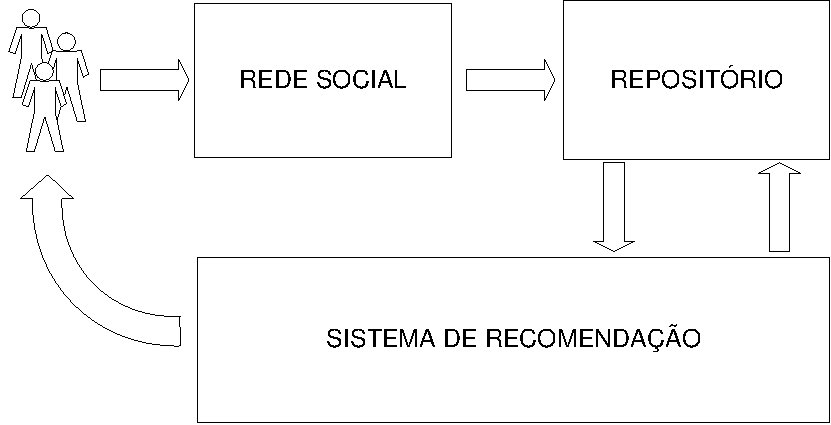
\includegraphics[width=\textwidth]{imagens/Diagrama_Visao_Geral}
  \caption{\it Diagrama de blocos do sistema}
  \label{fig:escopo}
\end{figure}

 Será realizado um experimento com 60 pessoas que se cadastrarão e formarão uma rede social disposta em 12 grupos de 5 amigos. O sistema de recomendação utilizará essa rede social para obter as informações de relações de amizade entre os usuários. Neste contexto, um usuário é considerado amigo do outro quando eles pertencem a um mesmo grupo de amigos. Os grupos de usuários são definidos a partir do envio de um e-mail com um convite de um usuário já cadastrado no sistema a outra pessoa. Este e-mail possui um endereço de cadastro, onde é possível a pessoa se cadastrar e automaticamente já fazer parte do grupo de amigos do usuário que a convidou.

 Os usuários poderão receber recomendações dos seus amigos ou de outras pessoas presentes na rede. Além disso, o sistema de recomendação utilizará informações de avaliações de produtos por parte dos usuários para poder recomendar outros produtos a eles. Como visto na Figura~\ref{fig:escopo}, os usuários entram com as informações na rede social, sendo estas utilizadas pelo sistema para a recomendação de produtos. O sistema de recomendação utilizará 3 tipos de algoritmos baseados em :

\begin{itemize}
	\item Similaridade entre perfis
	\item Similaridade de produtos
	\item Confiança
\end{itemize}

 Os dois primeiros são algoritmos conhecidos. A maioria dos sistema de recomendação se utilizam de algum deles ou de uma mistura dos dois. Ambos utilizam as avaliações dos usuários a produtos, para então poder recomendar outros produtos.

 O algoritmo de recomendação baseado em confiança utiliza as avaliações de produtos recomendados por usuários. Quando uma pessoa presente na rede social recomenda um produto a outra, a que recebe deve avaliar o produto recomendado. Essa avaliação é utilizada pelo sistema para calcular o grau de confiança que o usuário que recebe a recomendação tem no usuário que a realizou. Este grau de confiança é bidirecional, sendo que entre duas pessoas, uma pode ter um alto grau de confiança na outra, enquanto a outra tem um baixo de grau de confiança na primeira. Com estar informações, para recomendar produtos a uma pessoa, o sistema aplica o algoritmo de similaridade entre perfis apenas naquelas pessoas que já realizaram recomendações para ela, ou seja, apenas pessoas que têm informação de confiança são consideradas. Como dito anteriormente, para se ter informações de confiança, é necessário que uma pessoa recomende produtos a outra e que a pessoa que receba a recomendação, avalie o produto.
 
 A diferença entre o algoritmo baseado na similaridade entre perfis e no baseado em confiança está no fato de que apenas pessoas que recomendaram produtos são interessantes no cálculo. Além disso, quanto mais recomendações são realizadas entre duas pessoas, mais definido será o grau de confiança entre elas. O algoritmo de similaridade entre perfis considera todos os usuários presentes no sistema que avaliaram os mesmos produtos que a pessoa que receberá a recomendação. O algoritmo baseado em confiança utiliza esse alto grau de confiança que um usuário tem no outro para então conseguir recomendar bons produtos para o primeiro.

\section{Evolução do Projeto}

 O sistema que será utilizado no experimento está em fase final de elaboração. As pessoas que participarão já estão definidas, tendo todas concordado em participar e colaborar com a realização do experimento.

\subsection{Descrição do Experimento}
\label{cha:descricao_do_experimento}

 Inicialmente 12 pessoas serão convidadas a participar do experimento. Cada uma das 12 pessoas deverá convidar outras 4 pessoas para formarem um grupo de amigos. Sendo assim, formam-se 12 grupos de 5 amigos, totalizando 60 pessoas. Cada pessoa que participar de um grupo de amigos deverá concordar em ser definida como amiga de todos no grupo, ou seja, todas as pessoas pertencentes a um mesmo grupo de amigos se conhecem e se consideram amigas.

 Cada uma das 12 pessoas receberá 5 Termos de Consentimento Livre e Esclarecido (TCLE). Cada pessoa deverá receber um TCLE, lê-lo e assiná-lo. Após ler e assinar o TCLE a pessoa torna-se um participante do experimento e deve informar o seu e-mail para a pessoa que lhe convidou. De posse dos e-mails de todos presentes no grupo de amigos, cada uma das 12 pessoas deverá enviá-los aos pesquisadores.

 Um e-mail será enviado a cada um dos 60 participantes com um endereço da internet para que ele possa se cadastrar no sistema do experimento. Os grupos de amigos já serão formados no sistema com base nos endereços de e-mail enviados por cada uma das 12 pessoas que foram incialmente convidadas a participar. Os participantes deverão informar os seguintes dados no cadastro:

\begin{itemize}
	\item Nome
	\item Sexo
	\item Faixa etária (18-25, 26-30, 31-40, +40)
	\item Foto (Não obrigatório. Caso queira, o participante poderá escolher uma foto sua para representar o seu perfil no sistema.)
\end{itemize}

 Após isso, o participante deverá escolher a opção de salvar os seus dados e então será remetido a outra página do sistema que mostrará uma lista com 20 produtos escolhidos pelos pesquisadores. Tais produtos serão escolhidos com base na sua popularidade definida no site www.submarino.com (por exemplo, mais vendidos ou lançamento). O participante deverá avaliar TODOS os 20 produtos para passar para a próxima fase do experimento.

 Avaliar um produto significa dizer o quanto o participante acha aquele produto relevante para si, ou seja, o quanto ele se interessa pelo produto. A avaliação é feita por meio da atribuição de uma nota de 1 a 5, sendo 1 o participante não ter interesse e 5 o participante ter muito interesse naquele produto. Esse interesse não necessita ser um interesse de compra. O objetivo dessa avaliação é saber realmente o interesse do participante, podendo ser cobiça ou curiosidade, além de admiração pelo produto.

 Caso o participante não conheça o produto, ou seja, não tivesse ouvido falar dele ou não tivesse conhecimento suficiente para reconhecê-lo, até o instante em que ele lhe foi apresentado, ele deve escolher a opção "Não conheço". Mesmo não conhecendo, o participante deverá avaliar o produto de acordo com o seu grau de interesse. Essa avaliação será feita apenas com base na foto e descrição do produto.

 Terminadas as avaliações dos 20 produtos, o participante deverá procurar e avaliar - a avaliação deve ser feita da mesma forma como anteriormente - 10 produtos de sua escolha. Neste caso, o participante deverá avaliar apenas produtos de seu conhecimento, sendo que a opção de "Não conheço" não estará disponível.

 Os produtos poderão ser localizados a partir da filtragem de categorias e de um campo de busca por texto, onde o participante digita o nome do produto e o sistema o procura na base de dados, atualizando a lista com os resultados obtidos. As categorias de produtos presentes no sistema são:

\begin{itemize}
	\item Roupas
	\item Músicas
	\item Filmes
	\item Eletrônicos
	\item Livros
	\item Vinhos
	\item DVDs
	\item CDs
	\item Perfumes
\end{itemize}

 Para facilidade do participante, o sistema exibirá na tela o número de produtos restantes a serem avaliados.

 O sistema aguardará todos os participantes avaliarem os 20 produtos escolhidos pelos pesquisadores e os 10 produtos escolhidos por eles mesmos. Somente quando todos terminarem as etapas de avaliação de produtos que a etapa seguinte estará disponível. Esse sincronismo é necessitado pela próxima etapa. Neste meio tempo, o participante que já finalizou as suas tarefas receberá uma mensagem do sistema indicando que ele receberá um e-mail quando a próxima etapa estiver liberada.
 
 Na etapa seguinte, o sistema mostrará as fotos com o nome dos 4 amigos do grupo do participante e uma área com listagem aleatória de produtos cadastrados no sistema. Será solicitado ao participante que ele realize 5 recomendações a cada um dos quatro amigos do seu grupo, totalizando assim 20 recomendações a serem feitas. Para isso, o participante localiza um produto no sistema e escolhe a opção de recomendar a uma pessoa. Desse modo, será exibida a tela de recomendação de produto, com as informações do produto escolhido e uma lista com seus quatro amigos. O participante escolhe para quais amigos ele recomendará aquele produto e confirma a recomendação.
 
 O propósito das recomendações é que apenas boas recomendações sejam realizadas pelos participantes. Uma boa recomendação é a indicação de um produto que o participante acha que seu amigo achará interessante.

 Depois de fazer as 5 recomendações a cada amigo do seu grupo, o sistema mostrará ao participante uma lista contendo foto e nome de 10 participantes que não façam parte do seu grupo de amigos e solicitará a ele que recomende apenas 1 produto a cada uma dessas pessoas, totalizando 10 recomendações. Para poder fazer boas recomendações, o participante terá acesso às avaliações de produtos feitas por estas pessoas, além das informações de cadastro de cada uma delas. Para facilitar tal tarefa, o sistema indicará ao participantes quais das 10 pessoas ainda não receberam a sua recomendação.

 O sistema aguardará todos os participantes finalizarem as etapas de recomendar produtos aos amigos e aos desconhecidos antes de continuar o experimento. Neste meio tempo, o participante que já finalizou as suas tarefas visualizará no sistema uma mensagem indicando que ele receberá um e-mail quando a próxima etapa estiver liberada. Após a conclusão das etapas de recomendação por parte de todos os participantes, será enviado um e-mail a cada um deles avisando a continuidade do experimento.
 
 Ao entrar novamente no sistema o participante visualizará 20 recomendações de produtos. Estas são compostas de 5 recomendações feitas pelos seus amigos, 5 recomendações feitas por desconhecidos - em ambos os casos escolhidas aleatoriamente pelo sistema - e 10 recomendações feitas pelo sistema, cinco delas utilizando os algoritmos de recomendação com base em similaridade entre perfis e o restante similaridade entre produtos. O participante deverá avaliar o produto demonstrando o seu interesse na mesma escala de 1 a 5 utilizada para avaliar produtos anteriormente. A opção "Não conheço" está disponível nesta etapa. Não ficará visível ao participante quem é o autor da recomendação. Isso é feito para que não haja nenhuma influência sobre ele quando for avaliar o produto. Chamamos esta etapa de "teste cego". O sistema mostrará quantas recomendações restam para serem avaliadas pelo participante.
 
 Após avaliar as 20 recomendações, o participante receberá outras 30 recomendações. Neste caso serão utilizadas as 15 recomendações restantes realizadas pelos seus amigos, as 5 recomendações restantes feitas a ele por desconhecidos e 10 recomendações feitas pelo sistema utilizando o algoritmo de recomendação com base na confiança. Nesta etapa ficará visível ao participante quem é o autor da recomendação (inclusive quando for o sistema). Após terminar de avaliar todas as recomendações, o experimento será finalizado e uma mensagem de agradecimento será mostrada ao participante.

\section{Projeção da Análise dos Resultados}

\subsection{Dados Considerados}

 Após o término do experimento, serão considerados os seguintes dados extraídos do banco de dados do sistema:

\begin{itemize}
	\item Sexo e faixa etária dos usuários
	\item Grupos de usuários
	\item Avaliações dos produtos
	\item Recomendações realizadas por usuários
	\item Recomendações realizadas pelo sistema e o algoritmo que foi utilizado
\end{itemize}


\subsection{Medidas}

De posse de todos esses dados, serão realizadas as seguintes medidas.

\begin{itemize}

\item Erro na avaliação do produto

 Medir a diferença entre a avaliação prevista do produto pelo sistema e a avaliação dada pelo usuário. Quando o sistema recomenda um produto, ele calcula a avaliação prevista pelo usuário que receberá a recomendação.

\item Taxa de rejeição das recomendações
		
 Medir para cada usuário o número de recomendações que tiveram nota abaixo de 3 (1 ou 2). Fazer a relação com o total de recomendações recebidas por ele.

\item Taxa de serendipidade

 Medir o número de avaliações que contêm a informação "Não conheço" ativadas. Fazer a relação com o total de avaliações de produtos.

\item Grau de confiança calculado entre participantes do mesmo grupo

 Verificar o grau de confiança entre usuários do mesmo grupo e o grau de confiança da pessoa no sistema e nas pessoas desconhecidas que realizaram recomendação a ela.
\end{itemize}

 Os seguintes cenários serão considerados para a análise das medidas.

\begin{itemize}

\item Global

 Serão comparados os dados que envolvem todos os elementos presentes no sistema.

\item Grupo de amigos

 Serão comparados os dados apenas das pessoas que compõem um grupo de amigos. Todos os grupos serão analisados.

\item Algoritmos

 Neste cenário, iremos comparar os dados obtidos para os 3 diferentes tipos de algoritmo de recomendação utilizados no sistema.

\end{itemize}

 A análise será baseada em tabelas e gráficos construídos a partir dos dados retirados da base de dados do experimento.